%作者:王美庭
%Email:wangmeiting92@gmail.com

%使用xelatex或pdflatex编译

%=============导言区===============

\documentclass[compress,10pt,dvipsnames,notheorems]{beamer} %compress表示紧缩化显示slide;beamber会自动调用xcolor宏包,dvipsnames选项表示可使用xcolor宏包对应选项的颜色名;beamer会自动加载amsthm和amsmath宏包,notheorems表示关闭beamer定义的定理类环境。
% !TeX encoding = UTF-8
%作者:王美庭
%Email:wangmeiting92@gmail.com

%=============导言区通用设置===============

%%%=====主题设置*******
\usetheme{default} %设置整体上的主题
\usefonttheme[onlymath]{serif} %设置数学公式字体为衬线字体
\useoutertheme[subsection=false]{miniframes}
\useinnertheme{circles}
%\usecolortheme{wolverine}
\setbeamertemplate{navigation symbols}{} %移除所有的导航栏
\setbeamertemplate{caption}[numbered] %展示图表计数器
%\setbeamertemplate{footline}[text line]{\hfill\strut\insertframenumber{} / \inserttotalframenumber} %在页面右下角添加“当前帧数 / 总帧数”,\strut表示生成一个宽度为0,总高度等于行距的不可见支柱
\setbeamersize{text margin left=0.8cm, text margin right=0.8cm} %设置文字区域左右留白的宽度
\setbeamertemplate{itemize subitem}{--} %将无序列表的标志样式改为--(第二层)
%\setbeamertemplate{itemize item}[circle] %将无序列表的标志样式改为圆形(第一层)
%\setbeamertemplate{enumerate item}[circle] %将有序列表的标志样式改为圆形(第一层)
%\setbeamertemplate{section in toc}[circle] %设置section in toc为圆形包含数字


%%%=====宏包使用********
%\usepackage[space=true,hyperref,UTF8]{ctex} %支持中文,加入超链接宏包,设置UTF8编码
\usepackage{graphicx} %引入图片所需宏包
\graphicspath{{figures/}} %设置图像插入路径
\usepackage{lipsum} %可输入英文假文
\usepackage{ragged2e}
\justifying\let\raggedright\justifying %设置段落对齐方式为两端对齐
\usepackage{float} %其H参数可以让浮动环境不再浮动
\usepackage{array} %提供了更多的表格列说明符,以及修正了一些表格显示上的问题
\usepackage{booktabs} %以使用学术上常见的三线表命令
\usepackage{dcolumn} %可使用小数点对齐列说明符
\usepackage{setspace}
\setstretch{1} %设置行间距的因子(默认为1)
\usepackage{calligra} %手写字体
\usepackage[T1]{fontenc} %以实现更多的字体功能,如默认字体下的斜体加粗
\usepackage{ifthen}



%设置计数器
\newcounter{mycntthm} %设置新的计数器
\newcounter{mycntexam}
\setcounter{mycntthm}{0} %设定计数器默认值
\setcounter{mycntexam}{0}


%开关设置
\newcommand{\thmseriesnamestyle}{English} % Chinese 表示设置定理类名称为中文,English 表示设置定理类名称为英文
\newcommand{\thmseriesnumbering}{true} % true 表示对定理类环境进行编号,false 表示不对定理类环境进行编号

\ifthenelse{\equal{\thmseriesnamestyle}{Chinese}}{%
	\newcommand{\dfnname}{定义}
	\newcommand{\lemmaname}{引理}
	\renewcommand{\thmname}{定理}
	\newcommand{\coroname}{推论}
	\renewcommand{\proofname}{证明.}
	\newcommand{\examname}{例}
	\newcommand{\alertname}{注意}
}%
{%
	\newcommand{\dfnname}{Definition}
	\newcommand{\lemmaname}{Lemma}
	\renewcommand{\thmname}{Theorem}
	\newcommand{\coroname}{Corollary}
	\renewcommand{\proofname}{Proof.}
	\newcommand{\examname}{Example}
	\newcommand{\alertname}{Alert}
}

\ifthenelse{\equal{\thmseriesnumbering}{true}}{%
	\newcommand{\mycntthm}{\stepcounter{mycntthm}\themycntthm}
	\newcommand{\mycntexam}{\stepcounter{mycntexam}\themycntexam}
}%
{%
	\newcommand{\mycntthm}{}
	\newcommand{\mycntexam}{}
}


%自定义颜色
\colorlet{temp}{violet} %定义环境颜色
\colorlet{fgmyupdfncolor}{temp}
\colorlet{bgmyupdfncolor}{temp!20}
\colorlet{bgmylowdfncolor}{temp!10}
\setbeamercolor{myupdfncolor}{fg=fgmyupdfncolor,bg=bgmyupdfncolor}
\setbeamercolor{mylowdfncolor}{fg=black,bg=bgmylowdfncolor}

\definecolor{fgmyupthmcolor}{RGB}{51, 51, 178} %引理定理环境颜色
\definecolor{bgmyupthmcolor}{RGB}{214, 214, 239}
\definecolor{bgmylowthmcolor}{RGB}{234, 234, 247}
\setbeamercolor{myupthmcolor}{fg=fgmyupthmcolor,bg=bgmyupthmcolor}
\setbeamercolor{mylowthmcolor}{fg=black,bg=bgmylowthmcolor}

\colorlet{temp}{blue!70!orange} %推论环境颜色
\colorlet{fgmyupcorocolor}{temp}
\colorlet{bgmyupcorocolor}{temp!20}
\colorlet{bgmylowcorocolor}{temp!10}
\setbeamercolor{myupcorocolor}{fg=fgmyupcorocolor,bg=bgmyupcorocolor}
\setbeamercolor{mylowcorocolor}{fg=black,bg=bgmylowcorocolor}

\colorlet{temp}{lime!60!black} %证明环境颜色
\colorlet{fgmyupproofcolor}{temp}
\colorlet{bgmyupproofcolor}{temp!20}
\colorlet{bgmylowproofcolor}{temp!10}
\setbeamercolor{myupproofcolor}{fg=fgmyupproofcolor,bg=bgmyupproofcolor}
\setbeamercolor{mylowproofcolor}{fg=black,bg=bgmylowproofcolor}

\definecolor{fgmyupexamcolor}{RGB}{0, 127, 0} %例子环境颜色
\definecolor{bgmyupexamcolor}{RGB}{204, 229, 204}
\definecolor{bgmylowexamcolor}{RGB}{229, 242, 229}
\setbeamercolor{myupexamcolor}{fg=fgmyupexamcolor,bg=bgmyupexamcolor}
\setbeamercolor{mylowexamcolor}{fg=black,bg=bgmylowexamcolor}

\colorlet{temp}{red} %警示环境颜色
\colorlet{fgmyupalertcolor}{temp}
\colorlet{bgmyupalertcolor}{temp!20}
\colorlet{bgmylowalertcolor}{temp!10}
\setbeamercolor{myupalertcolor}{fg=fgmyupalertcolor,bg=bgmyupalertcolor}
\setbeamercolor{mylowalertcolor}{fg=black,bg=bgmylowalertcolor}


%自定义定理类环境
\newenvironment{dfn}[1][]%定义环境
{
	\begin{beamerboxesrounded}[upper=myupdfncolor,lower=mylowdfncolor,shadow]{\dfnname{} \mycntthm{} \ifthenelse{\equal{#1}{}}{}{(#1)}}\ifthenelse{\equal{\thmseriesnumbering}{true}}{\addtocounter{mycntthm}{-1}\refstepcounter{mycntthm}}{}
}%
{
	\end{beamerboxesrounded}
}

\newenvironment{lemma}[1][]%引理环境
{
	\begin{beamerboxesrounded}[upper=myupthmcolor,lower=mylowthmcolor,shadow]{\lemmaname{} \mycntthm{} \ifthenelse{\equal{#1}{}}{}{(#1)}}\ifthenelse{\equal{\thmseriesnumbering}{true}}{\addtocounter{mycntthm}{-1}\refstepcounter{mycntthm}}{}
}%
{
	\end{beamerboxesrounded}
}

\newenvironment{thm}[1][]%定理环境
{
	\begin{beamerboxesrounded}[upper=myupthmcolor,lower=mylowthmcolor,shadow]{\thmname{} \mycntthm{} \ifthenelse{\equal{#1}{}}{}{(#1)}}\ifthenelse{\equal{\thmseriesnumbering}{true}}{\addtocounter{mycntthm}{-1}\refstepcounter{mycntthm}}{}
}%
{
	\end{beamerboxesrounded}
}

\newenvironment{coro}[1][]%推论环境
{
	\begin{beamerboxesrounded}[upper=myupcorocolor,lower=mylowcorocolor,shadow]{\coroname{} \mycntthm{} \ifthenelse{\equal{#1}{}}{}{(#1)}}\ifthenelse{\equal{\thmseriesnumbering}{true}}{\addtocounter{mycntthm}{-1}\refstepcounter{mycntthm}}{}
}%
{
	\end{beamerboxesrounded}
}

\renewenvironment{proof}[1][]%证明环境
{
	\begin{beamerboxesrounded}[upper=myupproofcolor,lower=mylowproofcolor,shadow]{\proofname}
}%
{
	\hfill$\blacksquare$
	\end{beamerboxesrounded}
}

\newenvironment{exam}[1][]%例环境
{
	\begin{beamerboxesrounded}[upper=myupexamcolor,lower=mylowexamcolor,shadow]{\examname{} \mycntexam{} \ifthenelse{\equal{#1}{}}{}{(#1)}}\ifthenelse{\equal{\thmseriesnumbering}{true}}{\addtocounter{mycntexam}{-1}\refstepcounter{mycntexam}}{}
}%
{
	\end{beamerboxesrounded}
}

\newenvironment{solu}%解答环境
{
	\begin{beamercolorbox}[rounded=true,shadow=true]{mylowexamcolor}
}%
{
	\end{beamercolorbox}
}

\renewenvironment{alert}[1][]%警示环境
{
	\begin{beamerboxesrounded}[upper=myupalertcolor,lower=mylowalertcolor,shadow]{\alertname}
}%
{
	\end{beamerboxesrounded}
}
 %插入导言区设置


%标题页设置
\title[short title]{This is a long long long long long title}
\subtitle[short subtitle]{This is a subtitle}
\author[Meiting Wang]{Meiting Wang}
\institute[IESR-JNU]{
	\small Institute for Economic and Social Research \\ Jinan University
}

%有多位作者时:
%\author[Arthur, Doe] % (optional, for multiple authors)
%{A.~B.~Arthur\inst{1} \and J.~Doe\inst{2}}
%
%\institute[VFU] % (optional)
%{
%	\inst{1}%
%	Faculty of Physics\\
%	Very Famous University
%	\and
%	\inst{2}%
%	Faculty of Chemistry\\
%	Very Famous University
%}

\date[2021/3/6]{\today}




%=================正文区=================
\begin{document}

\begin{frame}[plain,noframenumbering] %标题页帧
	\titlepage
\end{frame}

{
%\setbeamertemplate{footline}{} %临时置空footline
\begin{frame}[noframenumbering]{Outline} %大纲,[pausesections]表示动态一步一步显示,[hideallsubsections]表示隐藏所有的subsection,[hideothersubsections]表示隐藏非当前节下的subsection,[currentsection]表示只正常显示current section,而虚化其他的section
	\tableofcontents[hideallsubsections]
\end{frame}
}

% 在每一section的开头插入以下内容
\AtBeginSection[]{ % 不对section*起作用
	{\setbeamertemplate{footline}{} %临时置空footline
	\begin{frame}[noframenumbering]{Current section}
		\tableofcontents[currentsection,hideothersubsections]
	\end{frame}}
}

\section{Theorem Environment}%---------------------

\begin{frame}{Theorem environment}
	\begin{dfn}
		This is a dfn env.
	\end{dfn}\vspace{\baselineskip}

	\begin{dfn}[This is a definition]\label{dfn:xxx}
		This is a dfn env.
	\end{dfn}\vspace{\baselineskip}

	\begin{lemma}
		This is a lemma env.
	\end{lemma}\vspace{\baselineskip}

	\begin{lemma}[This is a lemma]
		This is a lemma env.
	\end{lemma}\vspace{\baselineskip}

	\begin{thm}
		This is a sentence.
	\end{thm}
\end{frame}

\begin{frame}{Theorem environment (Continue)}
	\begin{thm}[This is a theorem]\label{thm:yyy}
		This is a sentence.
	\end{thm}\vspace{\baselineskip}

	\begin{coro}
		This is a coro env.
	\end{coro}\vspace{\baselineskip}

	\begin{coro}[This is a coro]
		This is a coro env.
	\end{coro}\vspace{\baselineskip}

	\begin{proof}
		This is a proof env.
	\end{proof}\vspace{\baselineskip}

	\begin{exam}
		This is a exam env.
	\end{exam}
\end{frame}

\begin{frame}{The Theorem Environment (Continue)}
	\begin{exam}[This is a exam]\label{exam:zzz}
		This is a exam env.
	\end{exam}\vspace{\baselineskip}

	\begin{solu}
		This is a solution env.
	\end{solu}\vspace{\baselineskip}

	\begin{alert}
		This is a alert env.
	\end{alert}
\end{frame}


\section{Chart Environment}%------------------------

\subsection{Table}

\begin{frame}{Table}
	\begin{table}[htbp]
		\centering
		\caption{Descriptive statistics 1}
		\begin{tabular}{l*{5}{>{$}c<{$}}}
			\toprule
			&\text{count}&\text{mean}&\text{sd}&\text{min}&\text{max}\\
			\midrule
			price       &          74&     6165.26&     2949.50&        3291&       15906\\
			mpg         &          74&       21.30&        5.79&          12&          41\\
			weight      &          74&     3019.46&      777.19&        1760&        4840\\
			\bottomrule
		\end{tabular}
	\end{table}

	\begin{table}[htbp]
		\centering
		\caption{Descriptive statistics 2}\label{tab:sumyy}
		\begin{tabular}{l>{$}c<{$}*{2}{D{.}{.}{-1}}*{2}{>{$}c<{$}}}
			\toprule
			&\text{count}&\multicolumn{1}{c}{mean}&\multicolumn{1}{c}{sd}&\text{min}&\text{max}\\
			\midrule
			price       &          74&     6165.26&     2949.50&        3291&       15906\\
			mpg         &          74&       21.30&        5.79&          12&          41\\
			weight      &          74&     3019.46&      777.19&        1760&        4840\\
			\bottomrule
		\end{tabular}
	\end{table}
\end{frame}

\subsection{Figure}

\begin{frame}{Figure}
	\begin{columns}
		\column[c]{0.49\textwidth}
		\begin{figure}[htbp]
			\centering
			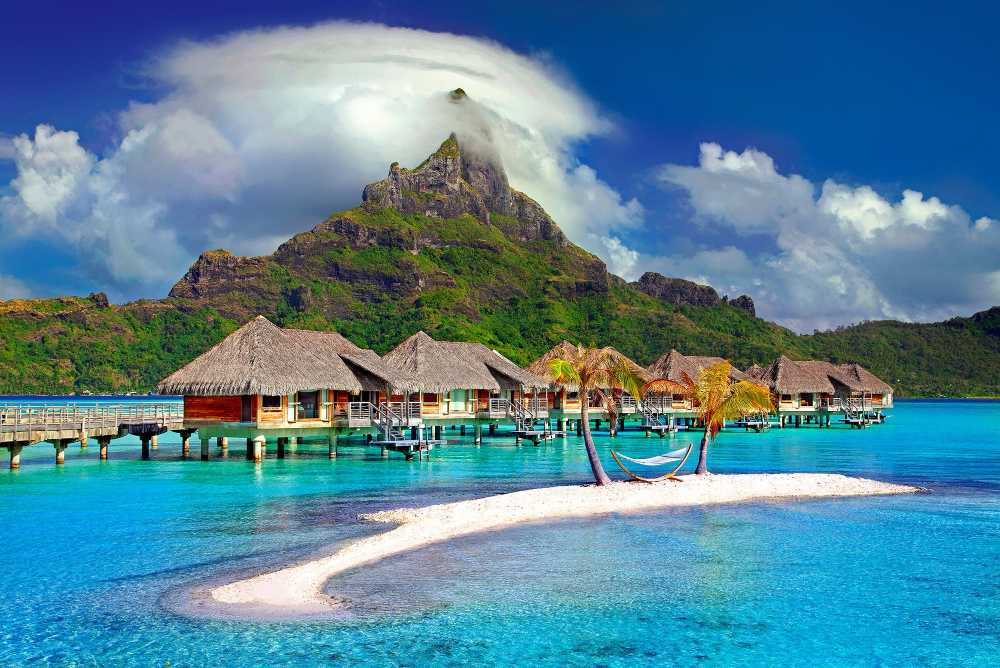
\includegraphics[width=\textwidth]{1.jpg}
			\caption{This is a figure 1}
		\end{figure}

		\column[c]{0.49\textwidth}
		\begin{figure}[htbp]
			\centering
			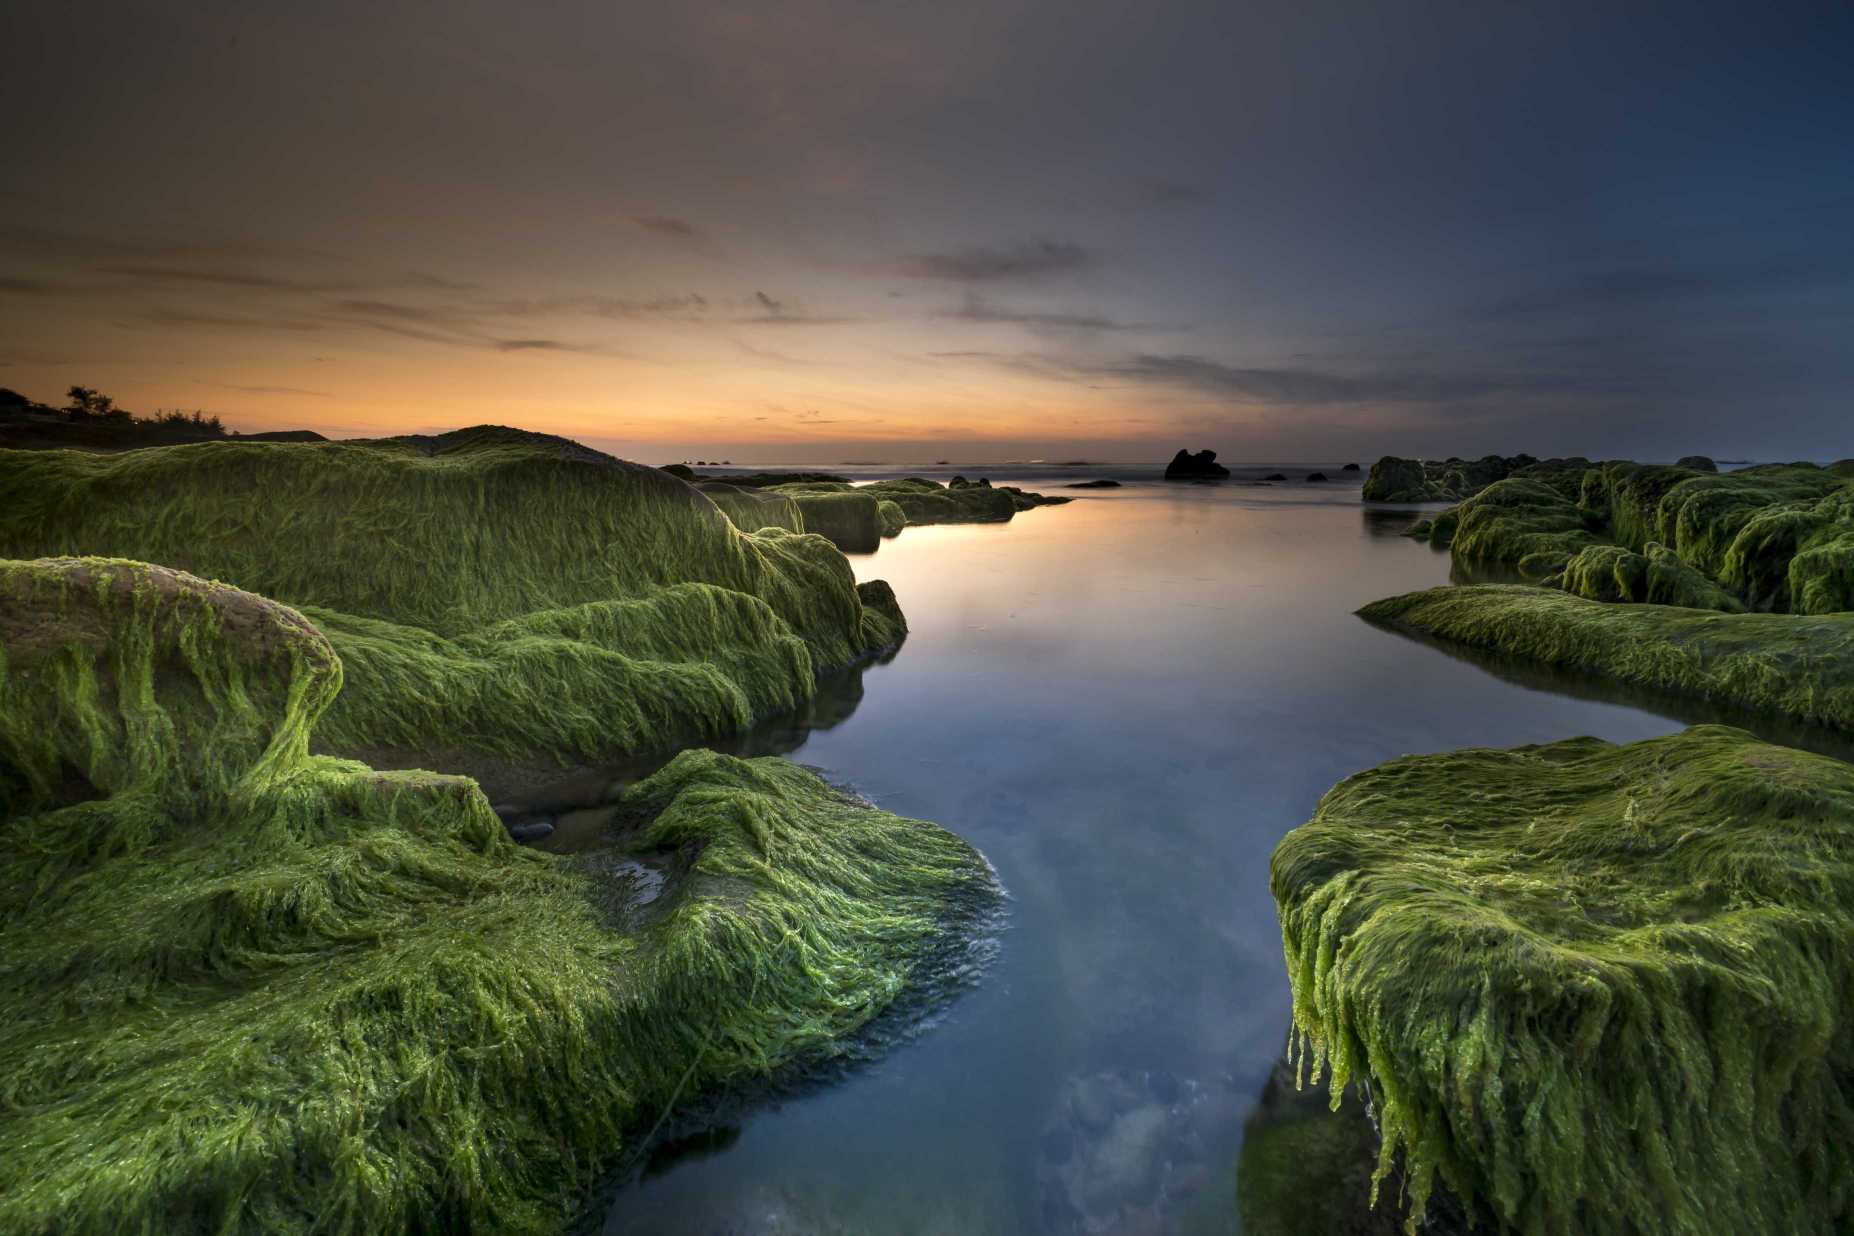
\includegraphics[width=\textwidth]{2.jpg}
			\caption{This is a figure 2}\label{fig:beauyy}
		\end{figure}
	\end{columns}
\end{frame}



\section{List Environment}%------------------------
\begin{frame}{List Environment} %可选项[c]表示将内容居中放置(也是默认的形式)
	\begin{columns}
		\column[c]{0.49\textwidth}
		\begin{itemize}
			\item The first item
			\begin{itemize}
				\item subitem 1
				\item subitem 2
			\end{itemize}
			\item The second item
			\item The third item
			\item The fourth item
		\end{itemize}

		\column[c]{0.49\textwidth}
		\begin{enumerate}
			\item The first item
			\begin{itemize}
				\item subitem 1
				\item subitem 2
			\end{itemize}
			\item The second item
			\item The third item
			\item The fourth item
		\end{enumerate}
	\end{columns}\vspace{2em}

	\begin{description}
		\item[First Item] Description of first item
		\item[Second Item] Description of second item
		\item[Third Item] Description of third item
	\end{description}
\end{frame}

\section{Mathematical Formula}%------------------------
\begin{frame}{Mathematical Formula}
	This is a one-row, unnumbered formula:
	\[ a^2 + b^2 = c^2 \]

	This is a one-line, numbered formula:
	\begin{equation}
		a^2 + b^2 = c^2
	\end{equation}

	There are multi-line, numbered formulas:
	\begin{gather}
		x = y + z \\
		y^2 = z + 6x \\
		z^2 + 6 = y^3 + x
	\end{gather}

	There are numbered formulas aligned at the equal sign:
	\begin{align}
		x^2 + x + 3 &= 9 \label{eq:alignx} \\
		x^3 + 9 &= x^2 + 5x \label{eq:aligny}
	\end{align}
\end{frame}

\section{Cross Reference}

\begin{frame}{Cross Reference}
	The use of cross references is shown below:
	\begin{itemize}
		\item There is a definition shown in \ref{dfn:xxx}.
		\item There is a theorem shown in \ref{thm:yyy}.
		\item There is a example shown in \ref{exam:zzz}.
		\item There is a formula shown in \eqref{eq:alignx}.
		\item There is a table shown in Table \ref{tab:sumyy}.
		\item There is a figure shown in Figure \ref{fig:beauyy}.
		\item The hyperlinks are contained in cross references above.
	\end{itemize}
\end{frame}

\section{Multi-column Environment}%------------------------

\begin{frame}{Multi-column Environment}
	\begin{columns}
		\column[c]{0.49\textwidth} %[c]垂直居中对齐,[t]垂直顶部对齐,[b]垂直底部对齐
		\lipsum[1][1-8]

		\column[c]{0.49\textwidth}
		\lipsum[3][1-3]
	\end{columns}
\end{frame}


\begin{frame}[plain,noframenumbering]
\vspace{0.12\textheight}\centering\Huge\textcalligra{Thanks!}\hspace{0em}
\end{frame}


\end{document}